% Portfolio-aligned résumé — compile with Tectonic (see latex/README.md)
% Section style: horizontal rule first, then heading (per layout request).
% Cyan link boxes: \fcolorbox{LinkCyan}{white}{...} inside \href (see \linkbox, \icontact, \projtitle).
%   Adjust: \definecolor{LinkCyan}{HTML}{...} and \LinkBoxRule for frame thickness.
% Source of truth for copy: src/features/portfolio/data.ts
\documentclass[10pt,a4paper]{article}

\usepackage[margin=0.6in]{geometry}
\usepackage{graphicx}
\usepackage[export]{adjustbox}
\usepackage{mathptmx}
\usepackage{xcolor}
\usepackage{enumitem}
\usepackage{array}
\usepackage{parskip}
\usepackage{tikz}
\usepackage{fontawesome5}
\usepackage[hidelinks]{hyperref}

% Near-black body; bright cyan frame around links (visual style similar to boxed link CVs)
\definecolor{ResumeHeading}{HTML}{020910}
\definecolor{ResumeAccent}{HTML}{082a5c}
\definecolor{ResumeMuted}{HTML}{151515}
\definecolor{ResumeBody}{HTML}{111111}
\definecolor{ResumeInk}{HTML}{000000}% pure black for emphasized headings / key labels
\definecolor{LinkCyan}{HTML}{00D4EA}

\hypersetup{
  colorlinks=false,
  pdfborder={0 0 0},
  pdfauthor={Prajwal B R},
  pdftitle={Prajwal B R — Résumé},
}

\newcommand{\LinkBoxRule}{0.48pt}
% Clickable link = thin cyan rectangle (drawn; works in every PDF viewer)
\newcommand{\linkbox}[2]{%
  \href{#1}{%
    \begingroup
    \setlength{\fboxsep}{3.2pt}%
    \setlength{\fboxrule}{\LinkBoxRule}%
    \fcolorbox{LinkCyan}{white}{\color{ResumeBody}#2}%
    \endgroup
  }%
}
\newcommand{\linkboxsmall}[2]{%
  \href{#1}{%
    \begingroup
    \small
    \setlength{\fboxsep}{2.8pt}%
    \setlength{\fboxrule}{\LinkBoxRule}%
    \fcolorbox{LinkCyan}{white}{\color{ResumeBody}#2}%
    \endgroup
  }%
}

\newcommand{\topic}[1]{\textbf{\textcolor{black}{#1}}}
\newcommand{\keypt}[1]{\textbf{\textcolor{black}{#1}}}
\newcommand{\projtitle}[2]{%
  \href{https://github.com/PRAJWAL-BR-0304/#1}{%
    \begingroup
    \setlength{\fboxsep}{3pt}%
    \setlength{\fboxrule}{\LinkBoxRule}%
    \fcolorbox{LinkCyan}{white}{\bfseries\color{ResumeBody}#2}%
    \endgroup
  }%
}
\newcommand{\icontact}[3]{%
  \href{#2}{%
    \begingroup
    \small
    \setlength{\fboxsep}{3pt}%
    \setlength{\fboxrule}{\LinkBoxRule}%
    \fcolorbox{LinkCyan}{white}{\color{ResumeBody}#1\,#3}%
    \endgroup
  }%
}

\setlength{\parskip}{0.22em}
\newlength{\ExpLogoCol}
\setlength{\ExpLogoCol}{30pt}
\newlength{\PersonalLogoHt}
\newlength{\PersonalLogoTot}
\newlength{\GhHalf}
\newlength{\GhDiam}
\newlength{\GhRad}
\newlength{\GhIconHt}
% GitHub-style badge (white squircle + black disc + white \faGithub), links to profile
\newcommand{\PersonalGithubBadge}{%
  \settoheight{\PersonalLogoHt}{\Large\bfseries M}%
  \PersonalLogoTot=\dimexpr\PersonalLogoHt*126/100\relax
  \GhHalf=\dimexpr\PersonalLogoTot/2\relax
  \GhDiam=\dimexpr\PersonalLogoTot-4.4pt\relax
  \GhRad=\dimexpr\GhDiam/2\relax
  \GhIconHt=\dimexpr\GhDiam*48/100\relax
  \href{https://github.com/PRAJWAL-BR-0304}{%
    \adjustbox{valign=c,height=\PersonalLogoTot}{%
      \begin{tikzpicture}[baseline=(current bounding box.center)]
        \filldraw[fill=white, draw=black!18, line width=0.16pt, rounded corners=2.6pt]
          (-\GhHalf,-\GhHalf) rectangle (\GhHalf,\GhHalf);
        \fill[black] (0,0) circle[radius=\GhRad];
        \node[inner sep=0pt] at (0,0) {%
          \resizebox{!}{\GhIconHt}{\textcolor{white}{\faGithub}}%
        };
      \end{tikzpicture}%
    }%
  }%
}
% Live portfolio (Netlify): single cyan box — PB mark + “My Portfolio”, one link.
\newcommand{\DeploySiteRow}{%
  \settoheight{\PersonalLogoHt}{\Large\bfseries M}%
  \PersonalLogoTot=\dimexpr\PersonalLogoHt*126/100\relax
  \href{https://prajwalbr.netlify.app}{%
    \begingroup
    \small
    \setlength{\fboxsep}{3pt}%
    \setlength{\fboxrule}{\LinkBoxRule}%
    \fcolorbox{LinkCyan}{white}{%
      \color{ResumeBody}%
      \adjustbox{valign=c}{%
        \begin{tikzpicture}[baseline=(current bounding box.center)]
          \coordinate (sw) at (0,0);
          \coordinate (ne) at (\the\PersonalLogoTot,\the\PersonalLogoTot);
          \filldraw[fill=black!88, draw=black!22, line width=0.12pt, rounded corners=2.35pt] (sw) rectangle (ne);
          \path (sw) -- (ne) node[midway, text=white, inner sep=0pt, font=\sffamily\fontsize{5.5}{5.5}\selectfont\bfseries] {PB};
        \end{tikzpicture}%
      }%
      \hspace{0.4em}%
      My Portfolio%
    }%
    \endgroup
  }%
}
\newcommand{\ExpLogoImg}[1]{%
  \makebox[\ExpLogoCol][c]{\includegraphics[height=20pt,width=20pt,keepaspectratio]{#1}}%
}

\setlist[itemize]{leftmargin=1.2em, topsep=0.12em, itemsep=0.08em, parsep=0pt, partopsep=0pt}

% --- Section: rule on top, title below (heading after the line) ---
% Section titles: explicit black + bold + slightly larger (reads clearly vs ResumeBody gray)
\newcommand{\secmajor}[1]{%
  \par\addvspace{0.48em}%
  \noindent{\color{ResumeHeading}\rule{\linewidth}{2.2pt}}%
  \par\vspace{0.3em}%
  \noindent{\normalfont\Large\bfseries\textcolor{black}{\MakeUppercase{#1}}}%
  \par\vspace{0.36em}%
}
\newcommand{\secminor}[1]{%
  \par\addvspace{0.48em}%
  \noindent{\color{ResumeHeading}\rule{\linewidth}{2.2pt}}%
  \par\vspace{0.3em}%
  \noindent{\normalfont\Large\bfseries\textcolor{black}{#1}}%
  \par\vspace{0.36em}%
}

\begin{document}
\thispagestyle{empty}
\pagestyle{empty}
\color{ResumeBody}% default body text slightly softer than pure black

% ---------- Header ----------
\noindent
\begin{minipage}[c]{0.14\linewidth}
  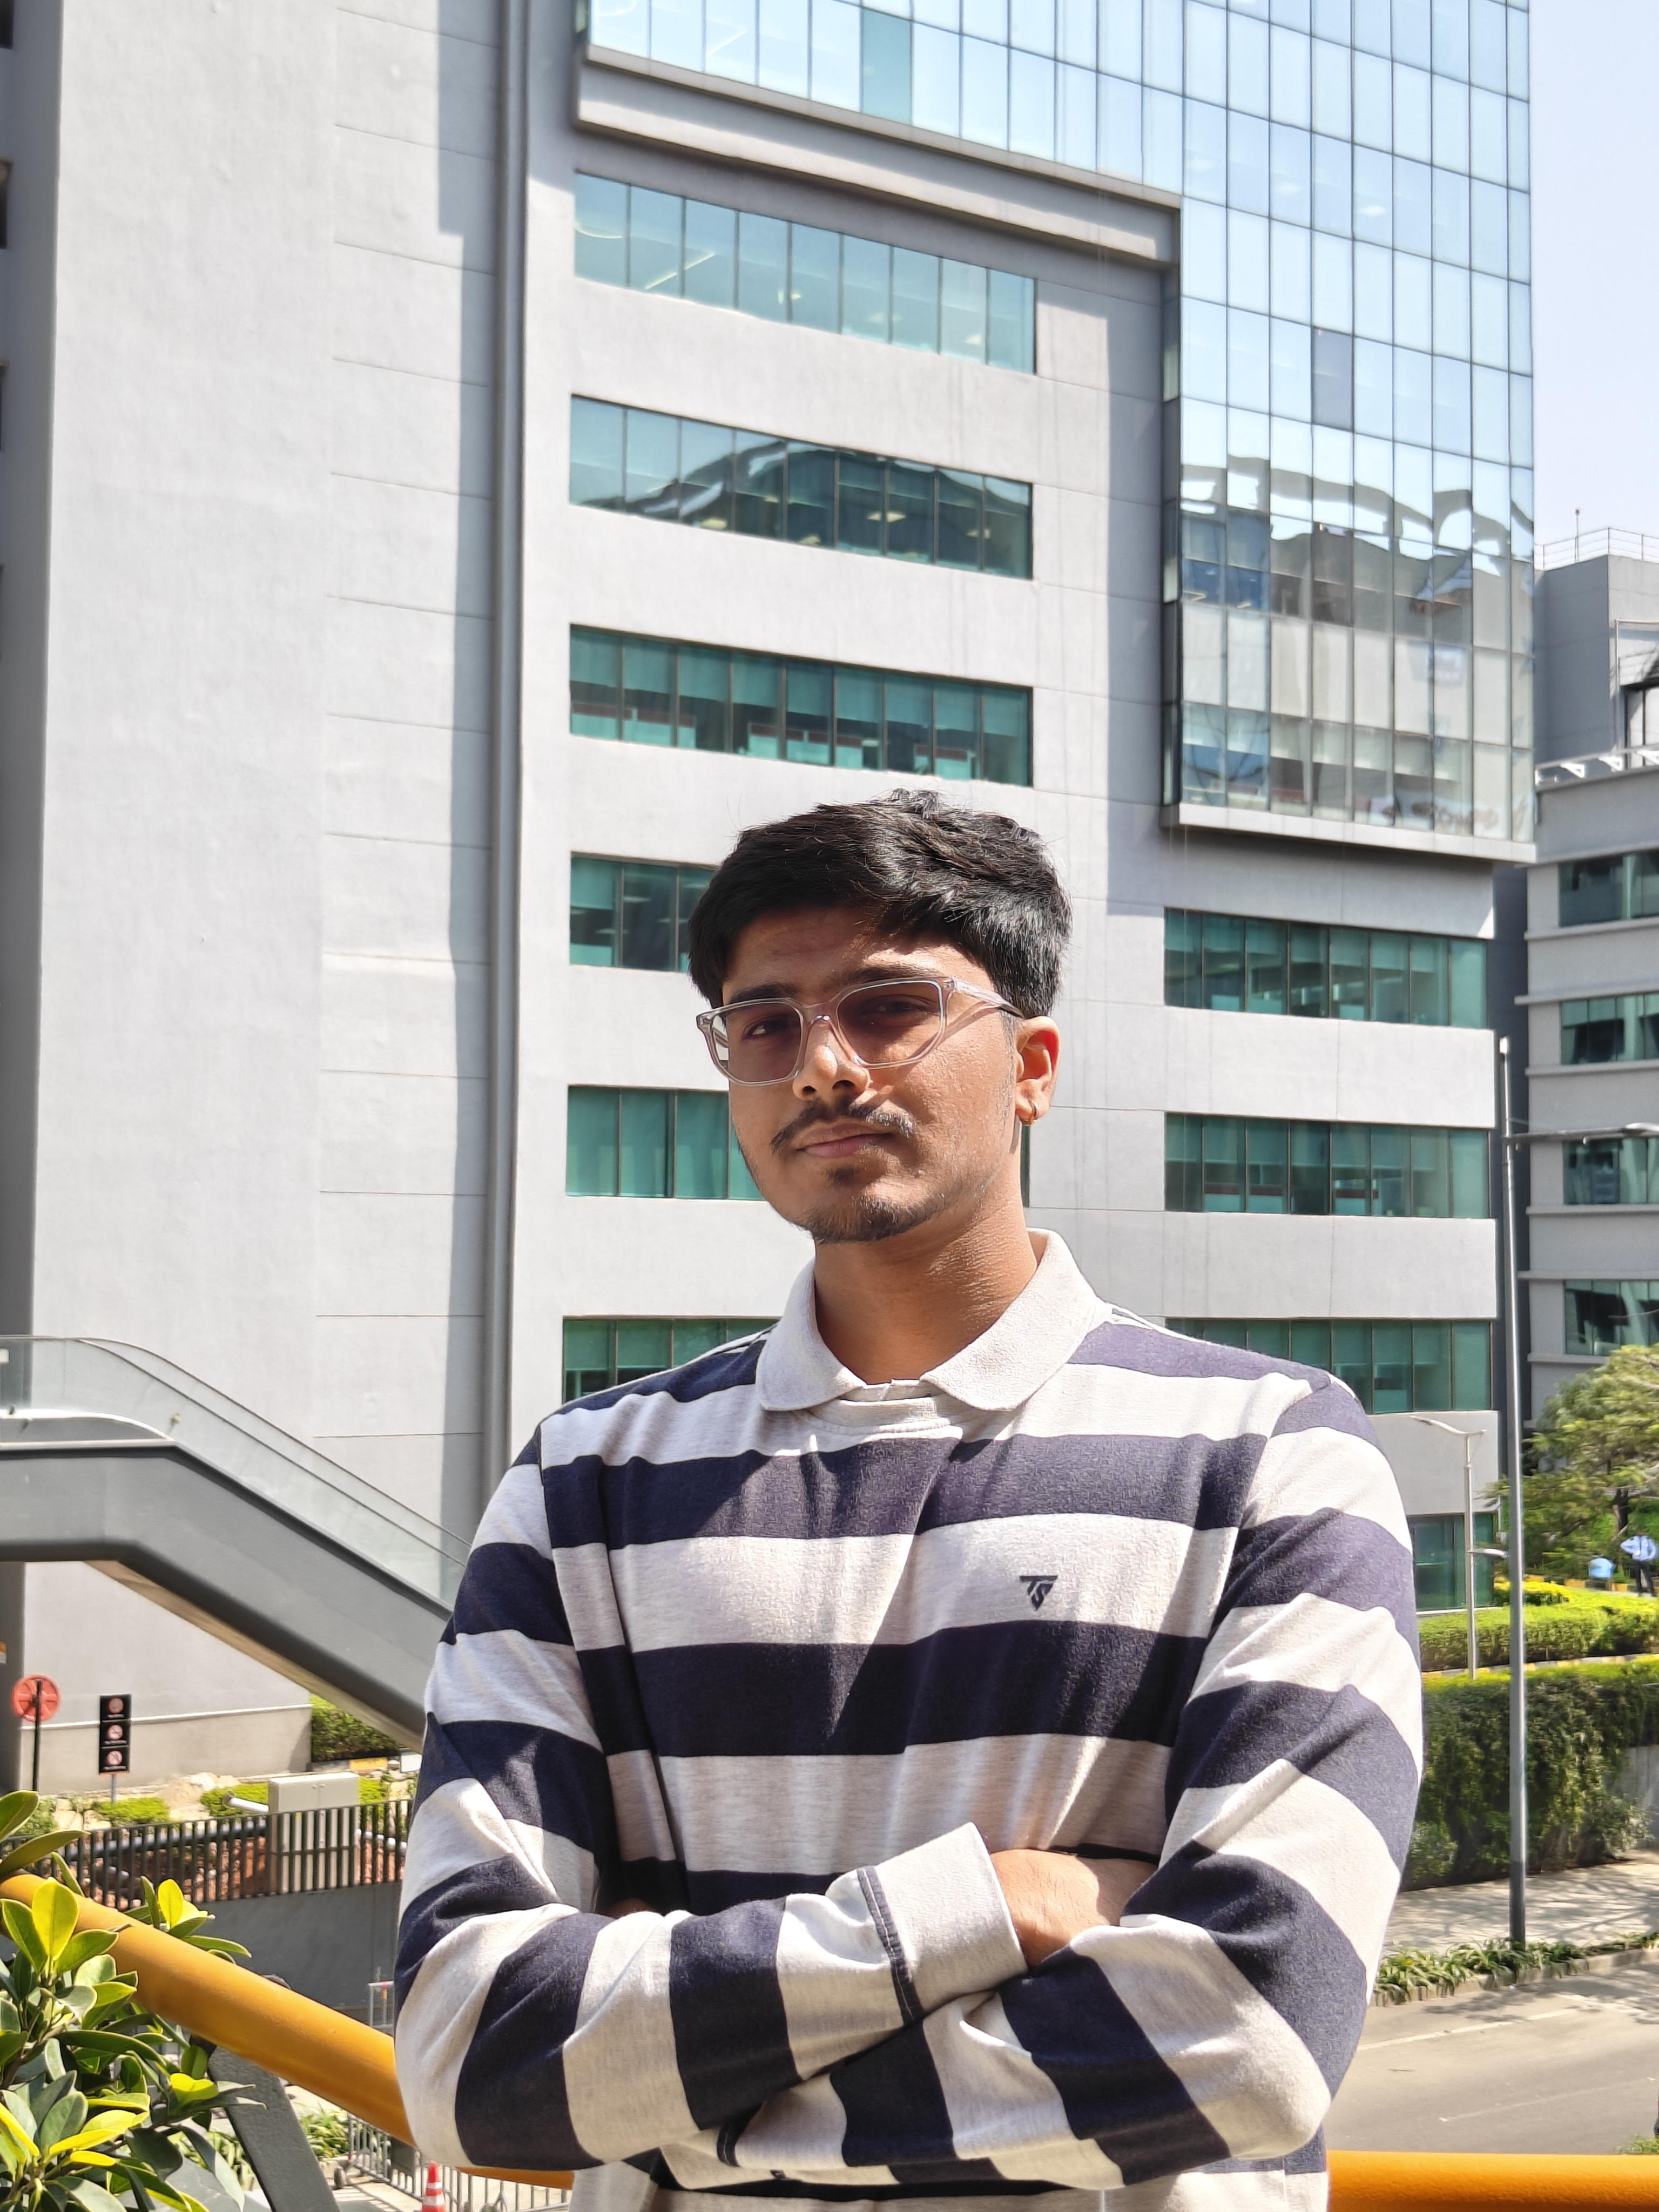
\includegraphics[width=\linewidth]{../public/images/profile.jpg}
\end{minipage}\hfill
\begin{minipage}[c]{0.82\linewidth}\raggedright
  {\LARGE\bfseries\textcolor{black}{Prajwal B R}}\\[0.16em]
  {\normalsize\bfseries Full-stack \& AI Developer}
  {\normalsize\itshape\color{ResumeMuted}\ --- Building real products with modern technology.}\\[0.24em]
  {\small Bengaluru, Karnataka, India \ \textbar\ \ %
  \textbf{\textcolor{black}{13+}} projects \ \textbar\ \ %
  \textbf{\textcolor{black}{15+}} GitHub repos \ \textbar\ \ %
  \textbf{\textcolor{black}{10+}} tech stacks}\\[0.32em]
  {\small
    \icontact{\faEnvelope}{mailto:prajwalbr0304@gmail.com}{prajwalbr0304@gmail.com}\\[0.1em]
    \icontact{\faGithub}{https://github.com/PRAJWAL-BR-0304}{github.com/PRAJWAL-BR-0304}
    \quad|\quad
    \icontact{\faLinkedin}{https://www.linkedin.com/in/prajwal-reddy-34024b307/}{linkedin.com/in/prajwal-reddy-34024b307}\\[0.1em]
    \DeploySiteRow
  }
\end{minipage}

\vspace{0.45em}

% ---------- PROFILE ----------
\secmajor{Profile}
{\small
Full-stack developer with hands-on experience shipping web and AI-backed products, blockchain integrations, and data-driven systems. Comfortable owning features end-to-end: API design, authentication, databases, cloud storage, and deployment pipelines. Currently focused on AI-native UX (streaming responses, tool use, guardrails), Web3 clients (MetaMask, testnets), and production-quality Next.js applications. Open to full-time roles, internships, and selective freelance engagements where impact is measurable.
}

% ---------- TECHNICAL SKILLS ----------
\secmajor{Technical skills}
{\small\raggedright
\begin{itemize}
  \item \topic{Languages \& runtimes:} TypeScript, JavaScript, Python, Java, C, SQL, HTML/CSS, Solidity, Dart (Flutter exposure).
  \item \topic{Web \& APIs:} Next.js, React, Vite, Tailwind CSS, Django, Django REST Framework, Flask, Express.js, Node.js, REST design, session- and JWT-style auth patterns.
  \item \topic{Data \& persistence:} PostgreSQL, MySQL, MongoDB, Supabase (Auth, RLS-aware clients), ORM/query modeling, file uploads to object storage (e.g.\ AWS S3).
  \item \topic{AI / LLM tooling:} OpenAI API, Groq, Gemini-oriented workflows, prompt engineering, retrieval-style patterns, streaming-first UIs (portfolio mirrors Vercel AI SDK-style flows).
  \item \topic{Blockchain \& Web3:} Ethereum/Sepolia testnets, MetaMask, ethers.js, contract-aware frontends, auction- and provenance-style dApp architecture.
  \item \topic{DevOps \& quality:} Git/GitHub, Docker, CI/CD collaboration (pipelines, regression automation), unit/integration testing, Playwright/Selenium familiarity.
\end{itemize}
}

% ---------- EXPERIENCE ----------
\secmajor{Experience}

\begingroup
\setlength{\tabcolsep}{0pt}%
\setlength{\arrayrulewidth}{0pt}%
% Logo: fixed-width box + slightly larger graphic; column widths avoid tabular* overflow (prevents logo orphan line)
% --- Nokia: logo vertically centered vs. two-line left block ---
\noindent
\begin{tabular*}{\linewidth}{@{}>{\centering\arraybackslash}m{\ExpLogoCol}@{\hspace{0.45em}}p{0.49\linewidth}@{\extracolsep{0pt plus 1fil}}>{\raggedleft\arraybackslash}p{0.26\linewidth}@{}}
  \ExpLogoImg{../public/images/experience/nokia-color-logo.png} &
  \begin{tabular}[t]{@{}l@{}}
    {\normalfont\large\bfseries\textcolor{black}{Nokia}}\\[0.14em]
    {\small\itshape\color{ResumeMuted}R\&D Engineer Intern}
  \end{tabular} &
  \begin{tabular}[t]{@{}r@{}}
    {\small\itshape\color{ResumeMuted}July 2025 --- Present}\\[0.14em]
    {\small\itshape\color{ResumeMuted}Bengaluru (On-site) --- OHUB}
  \end{tabular} \\
\end{tabular*}
\vspace{0.12em}
{\small\color{ResumeMuted}
\begin{itemize}
  \item Contribute to the \textbf{OHUB} initiative as part of \textbf{R\&D}: \textbf{backend services}, \textbf{internal APIs}, and integration points with existing Nokia platform tooling.
  \item Build and maintain \textbf{automation} for \textbf{build systems} and \textbf{regression checks}; shorten feedback loops for quality and release readiness.
  \item \textbf{Unit} and \textbf{integration testing}, structured test data for reproduction, and \textbf{CI/CD} pipeline hygiene alongside platform teams.
\end{itemize}
}

\vspace{0.42em}

% --- Personal projects: GitHub badge (not profile photo) + title; extra gap after icon ---
\begingroup
\noindent
\PersonalGithubBadge\hspace{0.58em}%
{\normalfont\Large\bfseries\textcolor{black}{Personal projects}}%
\hfill
{\small\itshape\color{ResumeMuted}2023 --- Present}\par
\vspace{0.12em}
{\small\color{ResumeMuted}
\begin{itemize}
  \item Shipped \keypt{13+} public repositories spanning \keypt{Next.js}, \keypt{Django}, \keypt{Solidity}, \keypt{Flask}, and \keypt{AI APIs}---from blockchain supply chains to \keypt{Groq}-powered knowledge bases.
  \item \keypt{MediTrustChain}: pharmaceutical traceability stack (web + contracts + mobile) with emphasis on provenance and monitoring; \keypt{DeFi-Homes}: on-chain property bidding UX with wallet flows.
  \item \keypt{KNOWLEDGE-BASE} \& \keypt{AI-GRAMMAR}: practical LLM integrations (\keypt{auth}, \keypt{persistence}, streaming-friendly UI patterns) aligned with modern full-stack practice.
\end{itemize}
}
\endgroup
\endgroup

% ---------- PROJECTS ----------
\secmajor{Projects}

\setlength{\fboxsep}{5pt}%
\setlength{\fboxrule}{0.55pt}%
\fcolorbox{ResumeHeading!40}{blue!5}{%
  \parbox{\dimexpr\linewidth-2\fboxsep-2\fboxrule}{%
    \small\textbf{\textcolor{black}{Primary code host:}}\ %
    \linkboxsmall{https://github.com/PRAJWAL-BR-0304}{\texttt{github.com/PRAJWAL-BR-0304}}%
  }%
}
\vspace{0.22em}

{\small
\setlength{\parskip}{0.35em}

\noindent\projtitle{MediTrustChain}{MediTrustChain}\quad
{\color{ResumeMuted}\textit{Next.js, TypeScript, Solidity (Sepolia), Supabase, Flutter; traceability, anomaly detection, GPS-aware flows.}}
\begin{itemize}
  \item Blockchain-based pharmaceutical supply chain with real-time traceability and AI-assisted anomaly detection to strengthen provenance narratives.
  \item Multi-surface delivery (web + Flutter) with managed backend/auth patterns suitable for regulated, audit-friendly workflows.
\end{itemize}

\noindent\projtitle{DeFi-Homes}{DeFi-Homes}\quad
{\color{ResumeMuted}\textit{React, Vite, TypeScript, Tailwind, Supabase, MetaMask, ethers.js, Chart.js, Framer Motion.}}
\begin{itemize}
  \item Decentralized real-estate auction experience: wallet onboarding, on-chain bidding metaphors, and transparent market visualization.
  \item Bridges traditional property discovery with Web3 mechanics while keeping off-chain profile/listing data coherent in Supabase.
\end{itemize}

\noindent\projtitle{eden-thought}{eden-thought}\quad
{\color{ResumeMuted}\textit{Django, PostgreSQL, AWS S3, HTML/CSS/JS, Render-oriented deploy.}}
\begin{itemize}
  \item Secure journaling platform with authentication, full CRUD for thoughts, and profile media uploads to object storage.
  \item Production-minded configuration for cloud databases and deployment templates suitable for hobby-to-demo scale traffic.
\end{itemize}

\noindent\projtitle{KNOWLEDGE-BASE}{KNOWLEDGE-BASE}\quad
{\color{ResumeMuted}\textit{React, Vite, TypeScript, Supabase, Groq; Markdown rendering.}}
\begin{itemize}
  \item Knowledge management with Supabase authentication and Groq-backed generation to produce and render Markdown pages on demand.
  \item Demonstrates practical RAG-adjacent UX: fast iteration loops, clear loading states, and server-brokered model access.
\end{itemize}

\noindent\projtitle{AI-GRAMMAR}{AI-GRAMMAR}\quad
{\color{ResumeMuted}\textit{Node.js, Express, EJS, Bootstrap, OpenAI (GPT-4o-mini).}}
\begin{itemize}
  \item Paste-in grammar correction workflow with server-side API usage patterns and a clean, form-driven UI.
  \item Useful baseline for comparing prompt strategies and safe-by-default key handling in small apps.
\end{itemize}

\noindent\projtitle{Student-Management-System}{Student-Management-System}\quad
{\color{ResumeMuted}\textit{Django~5, RBAC dashboards, attendance, leave, notifications.}}
\begin{itemize}
  \item Role-based portals for Admin, HOD, Staff, and Students with cohesive navigation and domain-specific workflows.
  \item Exercises realistic school operations modeling beyond toy CRUD examples.
\end{itemize}

\noindent\projtitle{pdf-to-text-converter}{pdf-to-text-converter}\quad
{\color{ResumeMuted}\textit{Python, Flask, OCR.space, Docker; TXT/PDF export, optional email delivery.}}
\begin{itemize}
  \item Upload-to-text pipeline with native parsing paths and OCR fallback for scanned PDFs.
  \item Packaged with Docker and cloud deploy notes for repeatable environments.
\end{itemize}
}

% ---------- PUBLICATIONS ----------
\secminor{Publications}

{\small
\begin{itemize}
  \item \topic{MediTrustChain}\ --- Blockchain-Based Pharmaceutical Supply Chain Traceability with AI-Assisted Anomaly Detection. \textit{ICAISE 2026}, Springer Nature proceedings (published)---on-chain provenance, monitoring, and AI-assisted anomaly signals for safer supply chains. \linkboxsmall{https://link.springer.com/chapter/10.1007/978-3-032-23547-3_23}{Publisher listing}
  \item \topic{DefiHomes}\ --- A Decentralized Real Estate Auction Platform with Transparent On-Chain Bidding. \textit{ICDMIS 2025}, Springer Nature LNNS (published)---smart-contract-centric bidding, escrow-style flows, and auditable histories for property markets. \linkboxsmall{https://link.springer.com/book/10.1007/978-3-032-25955-4}{Publisher listing}
  \item \topic{Smart Cradle}\ --- Secured Assistance and Monitoring System for Babies Using IoT. \textit{IEEE} conference publication---sensor-driven infant monitoring with connectivity patterns suited to caregiver alerting. \linkboxsmall{https://ieeexplore.ieee.org/abstract/document/10823361}{IEEE Xplore}
\end{itemize}
}

% ---------- EDUCATION ----------
\secmajor{Education}

\noindent

\includegraphics[height=15pt,valign=c]{../public/images/dsu-logo.jpg}\hspace{0.45em}
{\large\bfseries\textcolor{black}{\MakeUppercase{Dayananda Sagar University}}}\hfill{\small\textbf{Bengaluru}}\\[0.1em]
\noindent\hfill{\small B.E.\ Computer Science \& Engineering\ \textemdash\ 2022--2026 (expected)}\\[-0.12em]
\noindent\hfill{\small\textbf{CGPA:} 8.91/10}\\[0.3em]
\noindent\linkboxsmall{https://prajwalbreducation.netlify.app}{\faLink\enspace Explore Education}

% ---------- CERTIFICATIONS ----------
\secmajor{Certifications}

{\small
\begin{itemize}
  \item \topic{Generative AI \& LLM Bootcamp}\ --- Udemy (Feb 2025): transformers intuition, prompting, RAG, tool use, and small shipped LLM apps (32h).
  \item \topic{Django 5 Full Stack Masterclass}\ --- Udemy (Apr 2025): models, DRF, auth, PostgreSQL, testing, deployment patterns (22h).
  \item \topic{The Complete Prompt Engineering Bootcamp}\ --- Udemy (Jan 2025): structured prompts, guardrails, evaluation, automation patterns (14.5h).
  \item \topic{Google Cloud \& Firebase}\ --- Jun 2025: IAM basics, Firestore modeling, Firebase Auth/Hosting, Cloud Run-oriented full-stack patterns.
  \item \topic{Amazon Bedrock \& Strands Agents SDK}\ --- Jul 2025: agentic workflows, tool calling, session memory, observability on AWS training track.
  \item \topic{IBM SkillsBuild --- AI Fundamentals}\ --- Dec 2024: ethics/terminology, supervised learning intro, responsible AI framing.
  \item \topic{Infosys Springboard --- Full Stack Development}\ --- May 2025: frontend components/routing/state with backend API integration and validation.
\end{itemize}
}

% ---------- LANGUAGES ----------
\secminor{Languages}

\begin{itemize}
  \item English (professional), Kannada, Hindi, Telugu.
\end{itemize}

\end{document}
